%%%%%%%%%%%%%%%%%%%%%%%%%%%%%%%%%%%%%%%%%%%%%%%%%%%%%%%%%%%%%%%%%%%%%%%%%%%%%%%%%%%%%%%%%%%%%%%%%%%%%%%%%%%%%%%%%%%%%%%%%%%%%%%%%%%%%%%%%%%%%%%%%%%%%%%%%%%
% This is just an example/guide for you to refer to when submitting manuscripts to Frontiers, it is not mandatory to use Frontiers .cls files nor frontiers.tex  %
% This will only generate the Manuscript, the final article will be typeset by Frontiers after acceptance.   
%                                              %
%                                                                                                                                                         %
% When submitting your files, remember to upload this *tex file, the pdf generated with it, the *bib file (if bibliography is not within the *tex) and all the figures.
%%%%%%%%%%%%%%%%%%%%%%%%%%%%%%%%%%%%%%%%%%%%%%%%%%%%%%%%%%%%%%%%%%%%%%%%%%%%%%%%%%%%%%%%%%%%%%%%%%%%%%%%%%%%%%%%%%%%%%%%%%%%%%%%%%%%%%%%%%%%%%%%%%%%%%%%%%%

%%% Version 3.4 Generated 2018/06/15 %%%
%%% You will need to have the following packages installed: datetime, fmtcount, etoolbox, fcprefix, which are normally inlcuded in WinEdt. %%%
%%% In http://www.ctan.org/ you can find the packages and how to install them, if necessary. %%%
%%%  NB logo1.jpg is required in the path in order to correctly compile front page header %%%

\documentclass[utf8]{frontiersSCNS} % for Science, Engineering and Humanities and Social Sciences articles
%\documentclass[utf8]{frontiersHLTH} % for Health articles
%\documentclass[utf8]{frontiersFPHY} % for Physics and Applied Mathematics and Statistics articles

%\setcitestyle{square} % for Physics and Applied Mathematics and Statistics articles
\usepackage{url,hyperref,lineno,microtype,subcaption,booktabs,amssymb,amsmath,multirow,array}
\usepackage[onehalfspacing]{setspace}

\linenumbers


% Leave a blank line between paragraphs instead of using \\


\def\keyFont{\fontsize{8}{11}\helveticabold }
\def\firstAuthorLast{Amaya {et~al.}} %use et al only if is more than 1 author
\def\Authors{Jorge Amaya\,$^{1,*}$, Romain Dupuis\,$^{1}$, Maria-Elena Innocenti$^{2}$ and Giovanni Lapenta\,$^{1}$}
% Affiliations should be keyed to the author's name with superscript numbers and be listed as follows: Laboratory, Institute, Department, Organization, City, State abbreviation (USA, Canada, Australia), and Country (without detailed address information such as city zip codes or street names).
% If one of the authors has a change of address, list the new address below the correspondence details using a superscript symbol and use the same symbol to indicate the author in the author list.
\def\Address{$^{1}$Centre for mathematical Plasma-Astrophysics, CmPA, Mathematics Department, KU Leuven, University of Leuven, Belgium \\
$^{2}$Jet Propulsion Laboratory, Interstellar and Heliospheric Physics Division, 4800 Oak Grove Dr, Pasadena, CA 91109, USA}
% The Corresponding Author should be marked with an asterisk
% Provide the exact contact address (this time including street name and city zip code) and email of the corresponding author
\def\corrAuthor{Jorge Amaya, Mathematics Department, Celestijnenlaan 200B, KU Leuven, 3001 Leuven, Belgium}

\def\corrEmail{jorge.amaya@kuleuven.be, jorgeluis.amaya@gmail.com}
\graphicspath{{figures/}}


\begin{document}

\onecolumn
\firstpage{1}

\title[Visualizing and Interpreting Solar Wind Classifications]{Visualizing and Interpreting Unsupervised Solar Wind Classifications} 

\author[\firstAuthorLast ]{\Authors} %This field will be automatically populated
\address{} %This field will be automatically populated
\correspondance{} %This field will be automatically populated

\extraAuth{}% If there are more than 1 corresponding author, comment this line and uncomment the next one.
%\extraAuth{corresponding Author2 \\ Laboratory X2, Institute X2, Department X2, Organization X2, Street X2, City X2 , State XX2 (only USA, Canada and Australia), Zip Code2, X2 Country X2, email2@uni2.edu}


\maketitle

\tiny{	
\textbf{Word count}: in text (10172), in headers (105), outside text (843). Number of floats/tables/figures: 14.
}

\begin{abstract}

%%% Leave the Abstract empty if your article does not require one, please see the Summary Table for full details.
\section{}
One of the goals of machine learning is to eliminate tedious and arduous repetitive work. The manual and semi-automatic classification of millions of hours of solar wind data from multiple missions can be replaced by automatic algorithms that can discover, in mountains of multi-dimensional data, the real differences in the solar wind properties. In this paper we present how unsupervised clustering techniques can be used to segregate different types of solar wind. We propose the use of advanced data reduction methods to pre-process the data, and we introduce the use of Self-Organizing Maps to visualize and interpret 14 years of ACE data. Finally, we show how these techniques can potentially be used to uncover hidden information, and how they compare with previous manual and automatic categorizations.

\tiny
 \keyFont{ \section{Keywords:} solar wind, ACE, Self-Organizing Maps, clustering, autoencoder, PCA, unsupervised, machine learning} %All article types: you may provide up to 8 keywords; at least 5 are mandatory.
\end{abstract}

\section{Introduction}
The effects of solar activity on the magnetic environment of the Earth have been observed since the publication of Edward Sabine's work in 1852 \citep{Sabine1852}. During almost two hundred years we have learned about the intimate connection between our star and the plasma environment of the Earth. Three main physical processes connect the Sun to us: the transfer of electromagnetic radiation, the transport of energetic particles, and the flow of solar wind. The later is a continuous stream of charged particles that carries the solar magnetic field out of the corona and into the interplanetary space.

The name `solar wind' was coined by Parker in 1958 because `the gross dynamical properties of the outward streaming gas [from the Sun] are hydrodynamic in character'\citep{Parker1958}. Over time we have learned that the wind also has many more complex properties. Initially, it was natural to classify the solar wind by defining a boundary between `fast' and `slow' winds \citep{Habbal1997}. The former has been associated with mean speed values of 750 km/s, while the later shows a limit at 500 km/s, where the compositional ratio (Fe/O) shows a break \citep{Feldman2005,Stakhiv2015}. The solar wind also carries information about its origins on the Sun. At certain solar distances the ion composition of the solar wind is expected to be frozen-in, reflecting the electron temperature in the corona and its region of origin \citep{Feldman2005,Zhao2009,Stakhiv2015}. These particles have multiple energies and show a variety of kinetic properties, including non-Maxwellian velocity distributions \citep{Pierrard2010,Matteini2012}.

The solar wind is also connected to the Sun by the Interplanetary Magnetic Field (IMF), thorough magnetic field lines directed towards the Sun, away from the Sun, or in the case of flux ropes connected at both ends \citep{Owens2016,Gosling2010}. The thin region where solar magnetic fields of opposite directions meet is called the Heliospherc Current Sheet (HCS). When a spacecraft crosses the HCS instruments onboard can detect the change in magnetic field direction as a 180$^\circ$ reversal. Changes in the flow properties are also observed around the HCS. This perturbed zone is called the Heliospheric Plasma Sheet (HPS), and the passage of the spacecraft from one side of the HPS to the other is known as a Sector Boundary Crossing (SBC) \citep{Winterhalter1994}. In spacecraft observations these are sometimes confused with Corotating Interaction Regions (CIR), which are zones of the solar wind where fast flows have caught up with slow downstream solar wind, compressing the plasma.

From the point of view of a spacecraft SBCs and CIRs can show similar sudden changes in the plasma properties. These two in turn are often grouped and mixed with other transient events, like Coronal Mass Ejections (CME) and Magnetic Clouds (MC). Since 1981 when \citep{Burlaga1981} described the propagation of MC behind an interplanetary shock, it was suspected that CMEs and MC where coupled. However, more recent studies show that CMEs observed near the Sun do not necessarily become MC, but instead `pressure pulses' \citep{Gopalswamy1998,Wu2006}.

Much more recently it has been revealed, by observations from Parker Solar Probe, that the properties of the solar wind can be drastically different closer to the Sun, were the plasma flow is more pristine and has not yet mixed with the interplanetary environment. Patches of large intermittent magnetic field reversals, associated with jets of plasma and enhanced Poynting flux, have been observed and named `switchbacks' \citep{Bale2019,Bandyopadhyay2020}.

The solar wind is thus not only an hydrodynamic flow, but a compressible mix of different populations of charged particles and electromagnetic fields that carry information of their solar origin (helmet streamer, coronal holes, filaments, solar active regions, etc.) and is the dominion of complex plasma interactions (ICMEs, MC, CIRs, SBCs, switchbacks).

To identify and study each one of these phenomena we have relied in the past on a manual search, identification and classification of spacecraft data. Multiple authors have created empirical methods of wind type identification based on in-situ satellite observations and remote imaging of the solar corona. Over the years the number and types of solar wind classes has changed, following our understanding of the complexity of heliospheric physics.

Solar wind classification serves three main roles:
\begin{enumerate}
	\item it is used for the characterization of its origins in the corona,
	\item to identify the conditions where the solar wind is geoeffective,
	\item to isolate different plasma populations in order to perform statistical analysis.
\end{enumerate}

Among these classifications we can include the original review work by \citep{Withbroe1986}, the impressive continuous inventory by \citep{Richardson2000,Richardson2010,Richardson2012}, and the detailed studies by \citep{Zhao2009} and \citep{Xu2015b}. These publications classify the solar wind based on its origins and on the transient events detected. Each system includes two, three or four classes, generally involving coronal-hole origins, CMEs, streamer belt origins and sector reversal regions.

We are moving now towards a new era of data analysis, where manual human intervention can be replaced by `intelligent' software. The trend has already started, with the work by \citep{Camporeale2017b} who used the \citep{Xu2015b} classes to train a Gaussian Process algorithm that autonomously assigns the solar wind to the proper class, and more recently by \citep{Roberts2020} who used unsupervised classification to perform a 4 and 8 class solar wind classification. Machine learning algorithms have been used in the past in other applications in solar physics \citep{Lundstedt1996,Qahwaji2008c,Ahmed2013c,Bobra2015,Bobra2016,Nishizuka2017c,Camporeale2018}, and astrophysics \citep{VanderPlas2012,Ntampaka2015,Hajian2015,Suveges2017,Bai2018,Bonjean2019}.

The most basic machine learning techniques learn using two methods: a) in supervised learning the algorithms are shown a group of inputs and outputs with the goal to find a non-linear relationship between them, b) in unsupervised learning the machine is presented with a cloud of multi-dimensional points that have to be autonomously categorized in different classes. This means that we can program the computer to learn about the different types of solar wind using the existing empirical classifications, or by allowing it to independently detect patterns in the solar wind properties.

In the present work we show how the second method, unsupervised classification, can be used to segregate different types of solar wind. In addition, we show how to visualize and interpret such results. The goal of this paper is to introduce the method to the community, the best use practices and the opportunities that such system can bring. We implement one specific type of classification, called Self-Organizing Maps, and we compare it to simpler classification techniques, showing that it can reveal hidden information in years of solar wind data.

In the next sections we present in detail the techniques of data processing (section \ref{sec:dataprocessing}), data dimension reduction (sections \ref{sec:reducpca} and \ref{sec:reducae}) and data clustering (section \ref{sec:clustering}) that we have used. We then present in detail the Self-Organizing Map technique and all its properties in section \ref{sec:som}. We show how to connect all of these parts together in section \ref{sec:fullarchi}, and finally we show how the full system can be used to study 14 years of solar wind data from the ACE spacecraft in section \ref{sec:results}.

\section{Materials and Methods}

\subsection{Data and Processing}
\label{sec:dataprocessing}
\subsubsection{Data Set Used}
The solar wind data used in this work was obtained by the Advanced Composition Explorer (ACE) spacecraft, during a period of 14 years, between 1998 and 2011. The data can be downloaded from the \href{ftp://mussel.srl.caltech.edu/pub/ace/level2/multi}{FTP servers of The ACE Science Center (ASC)}. The files in this repository correspond to a compilation of hourly average data from three instruments: MAG (Magnetometer), SWEPAM (Solar Wind Electron, Proton, and Alpha Monitor) and EPAM (Electron, Proton, and Alpha Monitor). A detailed description of the entries in this data set can be found in the \href{http://www.srl.caltech.edu/cgi-bin/dib/rundibviewmultil2/ACE/ASC/DATA/level2/multi}{ASC website} listed in section \ref{sec:repos}.

A total of 122712 data points are available. However, routine maintenance operations, low statistics, instrument saturation and instrument degradation produce gaps and errors in the data. The SWICS data includes a flag assessing the quality of the calculated plasma moments. We retain only `Good quality' entries. Our pre-processed data set contains a total of 72454 points.

\subsubsection{Additional Derived Features}
We created additional features for each entry, based on previous knowledge of the physical properties of the solar wind. Some are derived from the existing properties in the data set, others computed from statistical analysis of their evolution. We introduce here the additional `engineered' features included in our data set.

Multiple techniques have been proposed in the literature to identify ejecta, Interplanetary Coronal Mass Ejections (ICME), and solar wind origins in the ACE data. \citep{Zhao2009} suggest that, during solar cycle 23, three classes of solar wind can be identified using its speed, $V_{sw}$, and the oxygen ion charge state ratio, $O^{7+}/O^{6+}$. It has been shown that slow winds originating in coronal streamers correlate with high values of the charge state ratio and fast winds coming from coronal holes presents low values \citep{DAmicis2015}. Plasma formed in coronal loops associated with CMEs also show high values of the charge state ratio \citep{Xu2015b}. The classification boundaries of the `Zhao classification' are presented in Table \ref{tab:swtypes}.

\citep{Xu2015b} suggested an alternative four classes system based on the proton-specific entropy, $S_p = T_p/n_p^{2/3}$, the Alfv\'en speed, $V_A = B / (\mu_0 m_p n_p)^{1/2}$, and the expected proton temperature, $T_\text{exp} = (V_{sw}/258)^{3.113}$. The classification conditions based on these three parameters are also presented in Table \ref{tab:swtypes}. This solar wind discrimination system will be known in this manuscript as the Xu classification \citep{Xu2015b}. For each entry in the data set we have included the values of $S_p$, $V_A$, $T_\text{exp}$, and the solar wind type given by the two classification methods. Two of the classes, i.e. ICME/ejecta and coronal hole, are common to the Xu and Zhao classifications. The number given to each class is arbitrary, but the two common classes share the same identification.

Auxiliary variables, like the Alfv\'en Mach number ($M_A$) and the temperature ratio ($T_\text{exp}/T_p$), have also been included in the data set. These features have been selected as they are the main components of the Xu classification and we want to compare the automatic classification methods against empirical models.

In addition to these instantaneous quantities, we can perform statistical operations over a window of time of six hours, including values of the maximum, minimum, mean, standard deviation, variance, auto-correlation, and range. We expect to capture with these quantities transient events in the immediate solar wind upstream and downstream. These are a complement to the stationary solar wind parameters mentioned above and add some information about the temporal evolution of the plasma. The selection of the statistical parameters and the window of time is arbitrary and will require a closer examination in a future publication.

Two additional terms, which have been successfully used in the study of solar wind turbulence and wave characterization \citep{Zhao2018,Adhikari2020,Magyar2019,DAmicis2015}, are included here to account for additional time correlations. These are: the normalized cross-helicity, $\sigma_c$ eq. \eqref{eq:sigmac}, and the normalized residual energy, $\sigma_r$ eq. \eqref{eq:sigmar}, where $\boldsymbol{b} = \left(\boldsymbol{B}- \boldsymbol{\left<B\right>}\right)/(\mu_0m_pn_p)^{1/2}$ is the fluctuating magnetic field in Alfv\'en units, $\boldsymbol{v} = \boldsymbol{V_{sw}}- \boldsymbol{\left<V_{sw}\right>}$ is the fluctuating solar wind velocity, $\boldsymbol{z^\pm} = \boldsymbol{v} \pm \boldsymbol{b}$ are the Els\"asser variables \citep{PhysRev.79.183}, and $\left<.\right>$ denotes the averaging of quantities over the time window.

\begin{align}
\sigma_c & = 2 \left< \boldsymbol{b}\cdot\boldsymbol{v}\right>/\left<\boldsymbol{b}^2 + \boldsymbol{v}^2\right> \label{eq:sigmac} \\
\sigma_r & = 2 \left< \boldsymbol{z^+}\cdot\boldsymbol{z^-}\right>/\left<\boldsymbol{z^-}^2 + \boldsymbol{z^+}^2\right> \label{eq:sigmar}
\end{align}

Due to gaps in the data, some of the above quantities can not be obtained. We eliminate from the data set all entries for which the derived features presented in this section could not be calculated. This leaves a total of 51608 entries in the data set used in the present work.

To account for the differences in units and scale, each feature column $\boldsymbol{F}$ in the data set is normalized to values between 0 and 1, using: $\boldsymbol{f}=\left(\boldsymbol{F}-\min{\boldsymbol{F}}\right) /\left(\max{\boldsymbol{F}}-\min{\boldsymbol{F}}\right)$.

Not all the features might be useful and some of them can be strongly correlated. We do not perform here a detailed evaluation of the inter dependencies of the different features, and we leave that task for a future work. The present manuscript focuses on the description of the methodology and on the visualization and interpretation capabilities of unsupervised machine learning classification. We limit our work here to test two models that use a different number of features. These are listed in table \ref{tab:features} and named Amaya-21, and Roberts-8, in honor of the work done by \citep{Roberts2020}. As the name suggests each model uses respectively 21, and 8 features of the data set. 

\subsubsection{Complementary Data Catalogs}
We support the interpretation of our results using data from three solar wind event catalogs. The first is the well known Cane and Richardson catalog that contains information about ICMEs detected in the solar wind, ahead of the Earth \citep{Cane2003} \citep{Richardson2010} \footnote{\href{http://www.srl.caltech.edu/ACE/ASC/DATA/level3/icmetable2.htm}{Near-Earth Interplanetary Coronal Mass Ejections Since January 1996: http://www.srl.caltech.edu/ACE/ASC/DATA/level3/icmetable2.htm}}. We used the August 16, 2019 revision. As the authors state in their website, there is no spreadsheet or text version of this catalog and offline editing was necessary. We downloaded and re-formatted the catalog to use it in our application. The CSV file created has been made available in our repository. We call this, the Richardson and Cane catalog. 

The second catalog corresponds to the ACE List of Disturbances and Transients\footnote{\href{http://www.ssg.sr.unh.edu/mag/ace/ACElists/obs\_list.html}{ACE Lists of Disturbances and Transients: http://www.ssg.sr.unh.edu/mag/ace/ACElists/obs\_list.html}} produced by the University of New Hampshire. As in the previous case, the catalog is only available as an html webpage, so we have manually edited the file and extracted the catalog data into a file also available in our repository. This is hereafter referred to as the UNH catalog.

Finally, we also included data from the Shock Database\footnote{\href{https://www.cfa.harvard.edu/shocks/ac_master_data/}{Harvard-Smithsonian, Center for Astrophysics, Interplanetary Shock Database - ACE: https://www.cfa.harvard.edu/shocks/ac\_master\_data/}} maintained by Dr. Michael L. Stevens and Professor Justin C. Kasper at the Harvard-Smithsonian Center for Astrophysics. Once again we have gathered and edited multiple web-pages in a single file available in our repository. In this work this database will be known as the CfA catalog.

\subsection{Dimension Reduction and Clustering}
\subsubsection{Dimension Reduction using PCA}
\label{sec:reducpca}
Principal Component Analysis (PCA) is a mathematical tool used in data analysis to simplify and extract the most relevant features in a complex data set. This technique is used to create entries composed of linearly independent `principal components'. These are the eigenvectors of the covariance matrix $\Sigma$ applied to the centered data, eq.\eqref{eq:covariance}, ordered from the largest to the smallest eigenvalue, $\lambda_1 \ge \lambda_2 \ge ... \ge \lambda_n$, where $\overline{\boldsymbol{X}}$ is the mean value of each original feature, eq.\eqref{eq:xmean}. The projection of the data onto the principal component space ensures a maximal variance on the direction of the first component. Each subsequent principal component is orthogonal to the previous ones and points in the direction of maximal variance in the residual sub-space \citep{Shlens2014}.

\begin{align}
\overline{\boldsymbol{X}} & = \frac{1}{m} \sum_{i=1}^{m} \boldsymbol{X}_i \label{eq:xmean} \\
\Sigma & = \frac{1}{m} \sum_{i=1}^{m} \left( \boldsymbol{X}_i - \overline{\boldsymbol{X}} \right)\left( \boldsymbol{X}_i - \overline{\boldsymbol{X}} \right) \label{eq:covariance}
\end{align}

The PCA transformation creates as many components in the transformed space, $\boldsymbol{\tilde{X}}$, as features in the original data space $\boldsymbol{X}$. However, components with small eigenvalues belong to a dimension where the variance is so small that it is impossible to separate points in the data. It is a general practice in data reduction to keep only the first $k$ components that explain at least a significant portion of the total variance of the data, $\lambda_{i=1..k}/\text{Tr}(\Sigma) > \epsilon$. This allows for a selection of information that will effectively differentiate data points, and for a reduction of the amount of data to process during analysis. Many techniques have been suggested for the selection of the values of $k$ and the cut-off $\epsilon$ \citep{Rea2016}. We use the value of $k=3$ to simplify the comparison among the different models, but for a detailed study of the solar wind, if a PCA transformation is applied, it is important to use a fixed criteria for the selection of the cut-offs.

Fig. \ref{fig:dimreduc} (A) is a 3D scatter plot of all the data points, colored by the Xu classification, projected on the first three PCA components. The features used to create this figure are presented in section \ref{sec:fourmodels}. Panel (B) contains the same data colored by the Zhao classification. These projections show that the Xu and Zhao classification are defined by hyper-planes separating the points, even if the data has been linearly transformed by the PCA. Class 2, ICMEs-ejecta, is restricted to a small domain in this coordinate system (for both the Xu and Zhao classification). The lateral plots on panel (A) are 2D histograms of the point distribution on the three main PCA planes. They show that the concentration of points is not homogeneous and different zones can be isolated using unsupervised classification techniques. There is a clear segregation of points in the (1st,2nd)-component plane: as we will see in subsequent sections, one of the features of the solar wind presents a strong bimodal distribution that is prioritized by the PCA.

\subsubsection{Dimension Reduction Using Autoencoders}
\label{sec:reducae}
PCA has a limitation: the principal components are a linear combination of the original properties of the solar wind. An alternative to data reduction is the use of autoencoders (AE). These are machine learning techniques that can create non-linear combinations of the original features projected on a latent space with less dimensions \citep{Hinton2006}. This is accomplished by creating a system where an encoding function, $\phi$, maps the original data $\boldsymbol{X}$ to a latent space, $\boldsymbol{\mathcal{F}}$, eq.\eqref{eq:encoder}. A decoder function, $\psi$, then maps the latent space back to the original input space, eq.\eqref{eq:decoder}. The objective of the autoencoder is to minimize the error between the original data and the data produced by the compression-decompression procedure as shown in eq.\eqref{eq:aeminimization}.

\begin{align}
\phi: & \boldsymbol{X} \rightarrow \boldsymbol{\mathcal{F}} \label{eq:encoder}\\
\psi: & \boldsymbol{\mathcal{F}} \rightarrow \boldsymbol{X} \label{eq:decoder} \\
\phi,\psi = & \underset{\phi,\psi}{\arg \min} \left\lVert \boldsymbol{X} - (\phi \circ \psi) \boldsymbol{X} \right\rVert^2 \label{eq:aeminimization}
\end{align}

Autoencoders can be represented as feed-forward neural networks, where fully connected layers lead to a central bottleneck layer with few nodes and then expands to reach again the input layer size. An encoded element, $\boldsymbol{z} \in \boldsymbol{\mathcal{F}}$, can be obtained from a data entry, $\boldsymbol{x} \in \boldsymbol{X}$, following the standard neural network function, eq.\eqref{eq:encodex}, where $\boldsymbol{W}$ is the weights matrix, $\boldsymbol{b}$ is the bias, and $\sigma$ is the non-linear activation function.

\begin{align}
\boldsymbol{z} & = \sigma \left( \boldsymbol{W}\boldsymbol{x} + \boldsymbol{b} \right) \label{eq:encodex} \\
\boldsymbol{\hat{x}} & = \sigma' \left( \boldsymbol{W'}\boldsymbol{z} + \boldsymbol{b'} \right) \label{eq:decodez} \\ 
\mathcal{L}(\boldsymbol{x}, \boldsymbol{\hat{x}}) & =  \left\lVert \boldsymbol{x}- \boldsymbol{\hat{x}} \right\rVert^2 \label{eq:aeloss}
\end{align}

The decoding procedure, shown in eq.\eqref{eq:decodez}, transforms $\boldsymbol{z}\rightarrow\boldsymbol{\hat{x}}$, where the prime quantities are associated with the decoder. The loss function, $\mathcal{L}(\boldsymbol{x}, \boldsymbol{\hat{x}})$, is the objective to be minimized by the training of the neural network using gradient descent. Once training is completed, the vector $\boldsymbol{z}$ is a projection of the input vector $\boldsymbol{x}$ onto the lower dimensional space $\boldsymbol{\mathcal{F}}$.

Additional enhancements and variations of this simple autoencoder setup exist in the literature, including multiple regularization techniques to minimize over-fitting \citep{7407967}, Variational Autoencoders (VAE) that produce encoded Gaussian distribution functions \citep{Kingma2013}, and Generative Adversarial Networks (GAN) that produce new (unseen) data \citep{Goodfellow2014}. In this work we use the most basic form of autoencoders, presented above.

The second column of Fig.\ref{fig:dimreduc}, panels (C) and (
D), contains the same information as the first column, but with the data set encoded in the three dimensional latent space $\boldsymbol{\mathcal{F}}$. Panel (C) shows that all the classes in the Xu and Zhao classification are easy to distinguish, including ICMEs-ejecta (class 2) that is difficult to discern in the PCA. This projection also shows that class 4 from the Zhao classification in the bottom panels, overlaps with class 3 (sector reversal origin), and partially with class 2 (ejecta) in the Xu classification on the top panels. Panel (C) shows, on the side planes, 2D histograms of the density of points. These can be seen as the volume integral of the point density in each direction. Here again it is possible to observe multiple zones of high concentration, suggesting that multiple types of solar wind are present in the data and that they can be differentiated using an unsupervised classification technique. 

\subsubsection{Clustering Techniques}
\label{sec:clustering}
The goal of unsupervised machine learning is to group data points in a limited number of clusters in the N-dimensional space $\Omega\in\Bbb R^N$, where N is the number of features (components or properties) in the data set. Multiple techniques can be used to perform multi-dimensional clustering. We present in Fig. \ref{fig:clustering} the three clustering techniques used to classify our 3D reduced data. The panels in the first column show the data projected in the PCA reduced space, $\boldsymbol{\tilde{X}}$, while the second column shows the data in the latent AE space, $\boldsymbol{\mathcal{F}}$. Each row corresponds to a different clustering method. The colors in the top panels (A) and (D) were obtained using the $k$-means method \citep{1056489}, the colors in the middle panels (B) and (E) were obtained using the Gaussian Mixture Model (GMM) \citep{bishop2006machine}. The bottom panels are colored by the classes from the Self-Organizing Maps described later in section \ref{sec:som}.

The $k$-means technique has already been used in a recent publication for the determination of solar wind states \citep{Roberts2020}. To our knowledge other clustering methods have never been used in the literature to classify the solar wind, but \citep{Dupuis2020} has used the GMM to characterize magnetic reconnection regions in simulations using their velocity distribution information.

The colors used in Fig.\ref{fig:clustering} are assigned randomly by each clustering technique. The most glaring issue with them is that different methods can lead to different clusters of points. The GMM and the $k$-means agree on their classification in the PCA space, but show dissimilar results in the AE space. Moreover, for a single method, e.g. $k$-means, slight modifications of the clustering parameters, e.g. using a different seed for the random number generator, can lead to very different results. We address this last issue using an algorithm that launches the $k$-means and GMM algorithms 500 times until the methods converge to a quasi-steady set of clusters. But we warn that the results are implementation dependent.

In the present data set, the cloud of points is convex and well distributed in all three components. This raises one additional issue, observed more clearly in the first column of Fig.\ref{fig:clustering}: when classical clustering methods are applied to relatively homogeneously dense data, it divides the feature space in Vorono\"i regions with linear hyper-plane boundaries. This is an issue with all clustering techniques based on discrimination of groups using their relative distances (to a centroid or to the mean of the distribution). To avoid this problem density-based techniques, such as DBSCAN \citep{ester1996density}, and agglomeration clustering methods, use a different approach. However, we can not apply them here because in such homogeneous cloud of points these techniques lead to a trivial solution where all data points are assigned to a single class.

There is no guarantee that a single classification method, with a particular set of parameters will converge to a physically meaningful classification of the data if the points in the data do not have some level of separability, or have multiple zones of high density. This is also true for other classification methods based on `supervised learning'. In those applications same issues will be observed if the training data uses target classes derived from dense data clouds using simple hyper-plane boundaries, as done for the Zhao and Xu classes. An example of such application was published by \citep{Camporeale2017b}. The authors used the Xu classification to train a Gaussian Process classifier.

\subsubsection{Self-Organizing Maps}
\label{sec:som}

\paragraph{Classical SOM}

Following the definitions and notations by \citep{Villmann2006}, a class can be defined as $C_i\overset{\text{def}}{=} \{x\in\Omega | \Phi(x)=\boldsymbol{w}_i\}$, where $\Phi$ is a function from $\Omega$ to a finite subset of $k$ points $\{\boldsymbol{w}_i\in\Bbb R^N\}_{i=1..k}$. A cluster $C_i$ is then a partition of $\Omega$, and $\{\boldsymbol{w}_i\}$ are the code words (also known as nodes, weights or centroids) associated. The mapping from the data space to the code word set, $\Phi: \Omega\rightarrow\mathcal{W}$, is obtained by finding the closest neighbor between the points $\boldsymbol{x}$ and the code words $\boldsymbol{w}$, eq.\eqref{eq:winner}. The code word $\boldsymbol{w_s}$, the closest node to the input $\boldsymbol{x_s}$, is called the `winning element'. The class $C_i$ corresponds to a Vorono\"i region of $\Omega$ with center in $\boldsymbol{w}_i$.

\begin{equation}
\Phi: x \rightarrow  \underset{i\in\mathcal{N}}{\arg\min}\left( \left\lVert x - \boldsymbol{w}_i \right\rVert \right) \label{eq:winner}
\end{equation}

A Self-Organizing Map (SOM) also composed of structured nodes arranged in a lattice, and assigned to a fixed position $\boldsymbol{p}_i$ in $\Bbb R^q$, where $q$ is the dimension of the lattice (generally $q=2$). The map nodes are characterized by their associated code words. The SOM learns by adjusting the code words $\boldsymbol{w}_i$ as input data $x$ is presented.

The SOM is the ensemble of code words and nodes $A_i = \{ \boldsymbol{w}_i, \boldsymbol{p}_i\} \in (\Omega \times \Bbb R^q)$. For a particular entry $\boldsymbol{x_s}$, the code word $s \in \mathcal{N}$ is associated to the winning node $\boldsymbol{p_s}$ if the closest word to $\boldsymbol{x_s}$ is $\boldsymbol{w_s}$. At every iteration of the method, all code words of the SOM are shifted towards $x$ following the rule:

\begin{equation}
\Delta \boldsymbol{w}_i = \epsilon(t)h_\sigma(t,i,s)(x-\boldsymbol{w}_i) \label{eq:learnsom}
\end{equation}

with $h_\sigma(t,i,j)$ defined as the lattice neighbor function:

\begin{equation}
h_\sigma(t,i,j) = e^{-\frac{\left\lVert \boldsymbol{p}_i - \boldsymbol{p}_j \right\rVert^2}{2\sigma^2(t)}} \label{eq:neigsom}
\end{equation}

where $\epsilon(t)$ is the time dependent learning rate, eq.\eqref{eq:epsilon}, and $\sigma(t)$ is the time dependent lattice neighbor width, eq.\eqref{eq:sigma}. The training of the SOM is an iterative process where each data point in the data set is presented to the algorithm multiple times $t={0, 1,..,t_f}$. In these equations the subscript $0$ refers to initial values at $t=0$ and the subscript $f$ to values at $t=t_f$.

\begin{align}
\epsilon(t) & = \epsilon_0 \left(\frac{\epsilon_f}{\epsilon_0}\right)^{t/t_f} \label{eq:epsilon} \\
\sigma(t) & = \sigma_0 \left(\frac{\sigma_f}{\sigma_0}\right)^{t/t_f} \label{eq:sigma}
\end{align}

This procedure places the code words in the data space $\Omega$ in such a way that neighboring nodes in the lattice are also neighbors in the data space. The lattice can be presented as a $q$-dimensional image, called map, where nodes sharing similar properties are organized in close proximity.

The main metric for the evaluation of the SOM performance is called the quantization error:

\begin{equation}
Q_E = \frac{1}{M} \sum_{i=1}^M \left\lVert x_i - w_{x_i} \right\rVert
\end{equation}

where $M$, is the total number of entries in the data set.

Once the training of the SOM is finished, the code words $\boldsymbol{w}_i$ can be grouped together using any clustering technique, e.g. k-means. The nodes of the SOM with close properties will be made part of the same class. The classes thus created are an ensemble of Vorono\"i subspaces, allowing a complex non-linear partitioning of the data space $\Omega$.

The final number of clusters is an input of the algorithm, but can also be calculated autonomously. The Within Cluster Sum of Squares (WCSS) can be used as a metric of the compactness of the clustered nodes. As its name implies the WCSS is the sum of the squared distances from each node to their cluster point. If only one class is selected, the large spread of the nodes would produce a high WCSS. The lowest possible value of the WCSS is obtained for a very high number of classes, when the number of classes is equal to the number of nodes. But such extreme solution is also unpractical. The optimal number of clusters can be obtained using the Kneedle class number determination \citep{5961514}. In the present work we do not use this technique: we will perform comparisons with previous publications that propose a fixed number of solar wind types. We will explore the use of an automatic class number selection in a future publication.

\paragraph{Dynamic SOM}
The time dependence of the SOM training allows the code words $\boldsymbol{w}_i$ to reach steady coordinates by slowing down their movement over the iterations. Due to the minimization of the distance in eq.\eqref{eq:winner} code words tend to agglomerate around high density zones of the feature space. The Dynamic Self-Organizing Map (DSOM), introduced by \citep{Rougier2011}, eliminate the time dependence and allows to cover larger zones of the space outside of the high density regions.

The DSOM is a variation of the SOM where the learning function \eqref{eq:learnsom} and the neighbor function \eqref{eq:neigsom} are replaced by eqs. \eqref{eq:learndsom} and \eqref{eq:neigdsom} respectively:

\begin{align}
\Delta \boldsymbol{w}_i & = \epsilon \left\lVert x - \boldsymbol{w}_i \right\rVert_\Omega h_\eta(i,s,x)(x-\boldsymbol{w}_i) \label{eq:learndsom} \\
h_\eta(i,s,x) & = e^{-\frac{1}{\eta^2}\frac{\left\lVert \boldsymbol{p}_i - \boldsymbol{p}_j \right\rVert^2}{\left\lVert x - \boldsymbol{w}_s \right\rVert_\Omega^2}} \label{eq:neigdsom} 
\end{align}

where $\epsilon$ is a constant learning rate, $h_\eta(i,s,x)$ is defined as the new lattice neighbor function, and $\eta$ is the `elasticity' parameter. In their work \citep{Rougier2011} show that DSOM can be used to better sample the feature space $\Omega$, reducing the agglomeration of code words around high density zones. The DSOM does not converge to a steady solution, due to the lack of a temporal damping factor.

\paragraph{Visualization of SOM and DSOM}
Clustering techniques do not necessarily converge to a steady immutable solution. Differences in the training parameters or slight changes in the data can have an important impact on the final classification. These tools can be used for statistical analysis, comparisons, data visualization and training of supervised methods. But it will be practically impossible to claim the existence of a general objective set of states discovered only by the use of these basic clustering techniques.

However, SOMs and DSOMs provide an important tool for the study of the solar wind: the maps are composed of nodes that share similar properties with its immediate neighbors. This allows for visual identification of patterns and targeted statistical analysis.

We used the python package \href{https://github.com/JustGlowing/minisom}{MiniSom} \citep{vettigli2013minisom} as the starting point of our developments. Multiple methods of the MiniSom have been overloaded to implement the DSOM, and to use a lattice with hexagonal nodes. All auxiliary procedures used to calculate inter-nodal distances, node clustering, data-to-node mapping, and class boundary detection have been implemented by us. All visualization routines are original and have been developed using the python library Matplotlib \citep{hunter2007matplotlib}.

Fig.\ref{fig:maps} shows the basic types of plots and maps that can be generated using the SOM/DSOM techniques. This figure uses data from the model Amaya-21 which has been encoded, using AE, into a set of entries, $\boldsymbol{z}_i$, each one composed of three components. Panel (A) shows a histogram of the first two components of the feature space $\Omega$, with dots marking the position of the code words $\boldsymbol{w}_i$. The colors of the dots represent their SOM classification. The red lines connect a single code word $\boldsymbol{w}_s$ with its six closest neighbors. The panel (B) shows the `hit map' of the SOM. It contains the lattice nodes $\boldsymbol{p}_i$ associated to the code words $\boldsymbol{w}_i$. They are depicted as hexagons with sizes representing the number of data points connected to each node and colored by their SOM class. The thickness of the lines between lattice nodes represent the relative distance to its neighbors in the feature space $\Omega$. Red lines connect the node $\boldsymbol{p}_s$, associated to the code word $\boldsymbol{w}_s$ in panel (A), to its closest neighbors.

Panel (C) of Fig.\ref{fig:maps} corresponds to the value of a single feature associated to each node; as an example we use the ionized oxygen ratio $O^{7+}/O^{7+}$ (`O7to6'). To improve visualization all hexagon sizes have been set to their maximum and the inter-node distance line has been colored white. In order to obtain the correct value for each node, we must first perform a decoding of the data from the latent space, $\Omega=\boldsymbol{\mathcal{F}}$, to the original data set space, $\boldsymbol{X}$.

Panel (D) of Fig.\ref{fig:maps} shows that the nodes of the lattice can also be used to present data that has not been used in the training of the SOM. The method keeps track of the data set points associated to each lattice node, it is then possible to perform independent statistical operations on those points alone. Moreover, it is possible to activate the SOMs with just a subset of the data, i.e. with points that feature a specific solar wind type. In this case, as an example, we have colored the map using the average oxygen charge state $\left<Q_{O}\right>$ (`avqO'), and we have set the size of the nodes to represent the frequency of points with solar wind type Xu=2 (ejecta). The dark line between the lattice nodes designate the boundaries between different SOM classes.

These four representations are only a few examples of the variety of data that can be represented using SOMs. The most important aspect of the SOMs is that data is represented in simple 2D lattices where the nodes share properties with their neighbors. Here we also decided to use hexagonal nodes, connecting 6 equidistant nodes, but other types of representations are also valid, e.g. square or triangular nodes.

The bottom row of Fig.\ref{fig:maps} displays all three components of the code words $\boldsymbol{w}_i$ associated with each one of the $\boldsymbol{p}_i$ nodes. In the first panel they have been mapped to the basic colors Red, Green and Blue (RGB). The remaining panels have been colored using each individual component. The first panel is then the RGB composition of the three remaining ones where the boundaries between the SOM classes have been highlighted.

\subsubsection{The Full Architecture}
\label{sec:fullarchi}
The previous sections introduced all the individual pieces that we use for the present work. Here we give a global view of the full model. Fig.\ref{fig:architecture} shows how all the components are interconnected. The data set is composed of clean and processed entries. We tested the PCA transformation in cases Amaya-21 and Roberts-8, keeping only the first three principal components. This possible setup is presented on the left of the figure. It is also possible to perform an unsupervised clustering directly on the un-processed data, as shown on the top of the figure, but it is not recommended. For the remaining of this manuscript we present only the cases where the non-linear AE encoding, shown at the right of Fig.\ref{fig:architecture}. The bottleneck of the AE network is three nodes, i.e. the data is encoded in three components. The transformed data is then used to train the SOM.

After training, the code words of the SOM are then clustered to group together nodes that share similar properties. This second level classification is done using the $k$-means++ algorithm with 500 re-initializations (it is in general recommended to use between 100 and 1000 iterations). The total number of classes selected is an input of the model and has been set to 8. This arbitrary choice was made following the results presented by \citep{Roberts2020}. All the software was implemented in Python using as main libraries PyTroch \citep{paszke2019pytorch}, Scikit-learn \citep{pedregosa2011scikit}, Matplotlib \citep{hunter2007matplotlib}, MiniSom \citep{vettigli2013minisom}, Pandas \citep{mckinney2010} and NumPy \citep{oliphant2006guide}.

\paragraph{Autoencoder architecture}
We use a basic, fully connected feed-forward neural network for the encoding-decoding process. The bottleneck of the network has been fixed to three neurons in order to simplify the visualization. This arbitrary choice is another parameter of the models that need further investigation. The neural network is symmetric in size but the weights of the encoder, $\boldsymbol{W}$, and the decoder, $\boldsymbol{W'}$, are not synchronized (see eqs.\eqref{eq:encodex}, \eqref{eq:decodez}). We use multiple fully connected hidden layers, where the central layer is the size of the bottleneck. Each layer is composed of a linear regressor, followed by batch normalization and a ReLU activation function. The output layer of the network contains a linear regressor followed by a hyperbolic tangent activation function. The autoencoder has been coded in python using the PyTorch framework \citep{paszke2019pytorch}.

We use an Adam optimizer \citep{Kingma2014} for the gradient descent with a learning rate of 0.001 and a weight decay of 0.0001 for regularization. The loss function is the Mean Squared Error (MSE). We train the network for 30 epochs, after which we see no additional improvement in the loss function. The full data set was randomly divided 50\%/50\% between training and testing sets.

\paragraph{Two Models of Solar Wind Classification}
\label{sec:fourmodels}
We have tested the two models presented in Table \ref{tab:features}. The models are inspired by the work of \citep{Roberts2020}. We call these cases Amaya-21 and Roberts-8.  The table lists all the features used in each model. A detailed description of each feature can be found in the \href{http://www.srl.caltech.edu/cgi-bin/dib/rundibviewmultil2/ACE/ASC/DATA/level2/multi}{ACE Level 2 documentation}. To spread the data over a larger range of values in each component, we have used the logarithm of all the quantities, except of those marked with an asterisk in the table.

Features 15 to 20 contain an additional suffix, corresponding to a statistical operation performed on the corresponding feature. The operations include the mean, the range, the standard deviation and the auto-correlation of quantities over a window of time of 6 hours. This window allows to capture temporal (spatial) fluctuations in some of the solar wind parameters.

On the lower part of Table \ref{tab:features} we present the range of dates used for each model. For Amaya-21 we use the full data set, while for the model Roberts-8 we try to replicate as much as possible the choices made in \citep{Roberts2020}. The same table also contains the hyper-parameters selected to run the two models. The number of neurons per layer in the encoding half of the neural network is listed in the table and was manually selected to minimize the final loss value of the AE.

All the figures presented until now correspond to the processing of data from model Amaya-21. The amount of data and figures produced in this work is very large and is not possible to include all of them in the present document. We will present in the next section some highlights, but more detailed analysis of each one of the cases will be presented in future publications.

\paragraph{Budget}
Machine learning models require fine tuning of different parameters, from the selection and testing of multiple methods, to the parameterization of the final architecture. \citep{Dodge2019} suggests that every publication in machine learning should include a section on the budget used for the development and training of the method. The budget is the amount of resources used in the data processing, the selection of the model hyper-parameters (HP), and its training.

The most time-consuming task in the present work has been the data preparation, the model setup and debugging and the writing of the SOM visualization routines. All the techniques described in the previous sections have been coded in python and are freely accessible in the repositories listed in section \ref{sec:repos}. We estimate the effort to bring this work from scratch to a total of 2 persons month. Of these, one person week was dedicated to the manual testing an selection of different model HPs (autoencoder architecture, feature selection, learning rates, initialization methods, number of epochs for training, selection of data compression method, size of the time windows, etc.).

All classic clustering techniques presented in section \ref{sec:clustering} require only a few lines of code and can be trained in minutes on a mid-range workstation (e.g. Dell Precission T5600, featuring two Intel(R) Xeon(R) CPU E5-2643 0 @ 3.30GHz with four cores and eight threads each). The most time consuming tasks of our models are the training of the autoencoder (5\% of the total run time), the multiple passages of the clustering algorithms (15\% of the run time), and the optimization of the SOM hyper-parameters (80\% of the run time). The training of the SOM is performed in less than a minute.

For reference, the total run-time for each one of the models used in this work are: 60 minutes for the Amaya-21 model and 20 minutes for the Roberts-8 model.

\paragraph{Hyper-Parameter Optimization}
Our main goal in this manuscript is to introduce the use of the SOMs for the classification of solar wind data. SOMs require the selection of four main Hyper-Parameters (HPs): the size of the lattice, $(m\times n)$, the initial learning rate, $\epsilon_0$, and the initial neighbor radius, $\sigma_0$. In the case of the DSOM algorithm, these two last HPs are replaced by the constant learning rate, $\epsilon$, and the elasticity, $\eta$. The automatic selection of the best HP for machine learning model is called Hyper-Parameter Optimization (HPO).

We use the library `optuna' \citep{Akiba2019} to perform an automatic optimization of the four HPs. The optimization is based on a technique called Tree-structured Parzen Estimator (TPE) \citep{pmlr-v28-bergstra13}, which uses Bayesian Optimization to minimize a target function provided by the user. We propose the use of the objective function, $\mathcal{H}$, described in eq.\eqref{eq:hpo}:

\begin{equation}
\mathcal{H}\left(\sigma, \eta, m, n\right) = Q_E(\sigma, \eta, m, n) + \alpha \frac{m}{m_{max}} + \beta \frac{n}{n_{max}} + \gamma m n \label{eq:hpo}
\end{equation}

where $Q_E$ is the SOM quantization error, $m$ and $n$ are the number of lattice nodes in each dimension, and $m_{max}$ and $n_{max}$ are the given maximum number of possible nodes. The weight factors $\alpha$, $\beta$ and $\gamma$ are used to impose restictions on each term. We have fixed their value to $\alpha=\beta=0.4 Q_E^0$ and $\gamma=0.08Q_E^0$, where $Q_E^0$ is the quantization error at iteration zero of the first optimization trial. When a large number of nodes is available smaller values of $Q_E$ are automatically obtained because the mean distance from the data set entries to the code words is reduced. The second and third terms on the RHS of $\mathcal{H}$ leads the optimizer to reduce the number of nodes in the SOM. The squaring term $\gamma m n$ forces the map to be as squared as possible.

After a total of 100 trial runs of the model using different HPs, the optimizer selected the parameters presented in the lower section of table \ref{tab:features}. The total run time for the HPO of the case Amaya-21 is about 40 minutes. HPO is, understandably, one of the most expensive procedures in all our setup.

\section{Results and comparisons}
\label{sec:results}
\subsection{Interpretation of ACE data using SOMs}

\subsubsection{General overview}

Fig.\ref{fig:maps} (A) shows the distribution of code words in the latent space for the model Amaya-21. The feature and components maps in the bottom row show in addition that lattice nodes share common attributes with their neighbors. The regularity in the colors of the feature map confirms that the SOM keeps its most important feature: organization. This is clear by the proximity of neighboring code words in the latent space, marked with red lines. We expect then to find common patterns in all the following maps in this section.

In the same figure the panels (B) and (C), and the component maps in the bottom row, show black and white lines indicating the relative distances between the lattice nodes: thicker lines represent larger inter-node distances. This shows that there are sections of the map (groups of code words in the latent space) that can form separate groups. This group separation has been highlighted in the `Feature map': the $k$-means clustering of the code words divides the space following the inter-nodal divisions. The classified points in the 3D latent space are shown in the third row of Fig.\ref{fig:clustering}.

The `Hit map' in Fig.\ref{fig:maps} presents a good distribution of points among all the lattice nodes, except in regions isolated from the rest. These zones represents solar wind types that have atypical properties. One of the goals of the DSOM is to cover those isolated zones where rare events can be classified in separate nodes. In contrast, the classic SOM method tends to cluster the code words in regions of high density, troubling the categorization of rare events, like ICMEs, ejecta or magnetic clouds, in the solar wind data.

Fig.\ref{fig:datarange} shows the distribution of the SOM training data in the normalized range $\left[0..1\right]$. This is a violin plot superposed by a box plot, showing the data distribution for each one of the features listed in table \ref{tab:features}. Normalization of the data is performed using the maximum and minimum values of each feature, but outliers (extremely large or small values) can hinder the use of particular features. In any classification problem, outlier detection and elimination is extremely important. The figure shows that all our data points are well represented in the data. Even in some cases, like for feature 13 (Alfv\'en Mach number), where the distribution has a small width, it still covers a significant part of the total range. This figure also shows that feature 6 (cross-helicity, $\sigma_c$) has a bimodal distribution, with two peaks close to the limits. A significant part of the data lays close to the $\sigma_c = \pm 1$ limit. The cross-helicity is a measure of the Alfv\'enicity of the solar wind, representing the direction and intensity of the propagation of Alfv\'enic fluctuations. At the Earth orbit this is an indication of the origins of the solar wind in the north or south hemispheres of the Sun.

Feature 20 (Pearson auto-correlation of the magnetic field magnitude) also shows a large distribution function, with a marked peak near one. This quantity was calculated for a window of time of six hours and a time lag of one hour. It shows the extent to which the values of the magnetic field have changed in one hour. High autocorrelation values represent situations in which the magnetic field does not change during the window, i.e. values in the window at time $t$ are the same as values shifted by one hour, $t-1$. Completely uncorrelated signals, produced by random changes in time, will produce autocorrelation values close to 0 (0.5 after normalization), i.e. the data in the window at time $t$ is different from the data in the shifted window. Positive (negative) values represent a signal with a periodicity of one hour. Additional time lags could be used to create extra features, but here we use only one to test its effectiveness.

The features selected for this model have not followed a meticulous vetting process. We included features inspired from previous publications and new interesting additions. Our goal in this work was to test if the data transformation into an encoded latent space can account for redundant or un-interesting features. This is a very useful property for data sets where expert knowledge is not available. It also shows how the SOM can point to features that don't have added value. As we will see in the next sections, the method converges to meaningful classes, even when some of the features used turn out to be not very relevant. We will perform in a future publication a more detailed selection of the features, based on the experience of human experts. 

\subsubsection{Interpretation of the Automatic Classification}

Lattice nodes are characterized by their weights (code). Applying a reverse transformation, followed by a re-scaling, we obtain their values in the original N-dimensional space. Fig.\ref{fig:compmap} shows the DSOM clustering and the 21 solar wind properties associated to each lattice node. We have clustered the nodes in eight classes. This is a subjective selection inspired by other works in the literature. In our case the clustering leads to contiguous groups of nodes.

The maps show the properties that differentiate each of the eight classes. We can try to attribute a physical significance to the classes by analyzing, together, the characteristic features of each class in Fig.\ref{fig:compmap} and examples of the recorded solar wind data in Fig.\ref{fig:timeseries}. This figure presents a window of time of four months, from the beginning of May 2003 until the end of September 2003. We have plotted entries in the Richardson and Cane, UNH and CfA catalogs on top of time series of the solar wind speed in panels (A), (B) and (C). These plots have been colored by the class number of the $k$-means, GMM and SOM classes.

The polarity of the solar wind can be observed in panel (D). Changes from red to green are associated with crossings of the HCS. The z-component of the magnetic field is plotted in blue (positive) and red (negative) in panel (E).

Fig.\ref{fig:timeseries} (F) shows the evolution of the $O^{7+}/O^{6+}$ ratio using a dotted black line in logarithmic scale. The Zhao classification boundaries (see table \ref{tab:swtypes}) are plotted using a black continuous line. The red area corresponds to `non-coronal hole origin' solar wind, and data points receive this classification if the dotted line enters the red zone. If it stays above it, the solar wind is considered an ICME. If the curve drifts bellow the red zone, the wind is considered to have origins in a coronal-hole.

The three time series in panels (A), (B) and (C) show that multiple techniques can be used for the clustering of solar wind properties. But SOMs allow fast visualization and interpretation not available in other clustering methods. All time series have a strong tendency to group the solar wind in two groups, depending on the heliospheric sector. This is due to the importance of the cross-helicity in the data set and its bimodal distribution.

Class 5 can be easily mapped to ICMEs. It presents the very high $O^{7+}/O^{6+}$ ratio values that \citep{Zhao2009}, \citep{Stakhiv2015} and \citep{Xu2015b} associate to ICME plasma. It is also characterized by the high solar wind velocity, $\sigma_c \sim 0$ \citep{Roberts2020}, high values of magnetic field magnitude and Alfv\'en speed which are usually associated to explosive transient activity \citep{Xu2015b}. In Fig.\ref{fig:timeseries}, panel (C) shows that class 5 indeed maps well to the Richardson and Cane CME catalogs. We can use the cross-helicity, $\sigma_c$, to identify two groups of classes: the ones with mostly positive $\sigma_c$ (1 and 3) and mostly negative $\sigma_c$ (0, 2, 4, 6, 7). As already done in \citep{Roberts2020}, we associate them to plasma originated in areas with different magnetic field polarity, respectively ($B_x> B_y$) and ($B_y> B_x$). Additional inspection of Fig.\ref{fig:timeseries}, panels (C) and (D), confirms this association.

Among the classes with negative $\sigma_c$, class 7 can be quite confidently associated with coronal hole plasma. It is characterized by very low values of the $O^{7+}/O^{6+}$ ratio, associated with plasma originating from open magnetic field lines \citep{Zhao2009,Stakhiv2015}, high wind speed, low proton density and proton density variability, high absolute values of $\sigma_c$ and equipartition levels of $\sigma_r$ (telltale signs of Alfv\'enicity), high proton entropy and moderately high values of Alfv\'en speed (associate by \citep{Xu2015b} to coronal holes), high proton temperature and high proton temperature variability. Inspection of Fig.\ref{fig:timeseries} (C) supports this identification.

Class 4 and 0 are both possibly composed of a mix of slow Alfv\'enic wind \citep{DAmicis2015} and winds with conventional slow and intermediate speeds. The two classes share a possible coronal hole origin and a number of characteristics also associated with fast Alfv\'enic wind ($O^{7+}/O^{6+}$ ratio, low density values, high $\left\lVert \sigma_c \right\rVert$ and low $\sigma_r$ values). The main difference between fast and slow Alfv\'enic wind, apart from the speed, is the proton temperature, which tends to be lower in Alfv\'enic and `conventional' slow wind with respect to the fast wind.
 
The parameters that are normally used to distinguish between slow and fast wind (speed, density, proton entropy, proton temperature) span a quite large interval in classes 0 and 4, and in fact point to the presence of a mix of slow and fast wind. The main difference between the two classes is given by the very high values of residual energy $\sigma_r$ in class 4, which points to kinetically dominated structures.

Class 6 is characterized by features generally associated with intermediate and slow wind of streamer belt origin: intermediate values of $O^{7+}/O^{6+}$, intermediate and slow speed, high proton density, low absolute value of cross-helicity, low values of magnetic field magnitude, proton entropy, Alfv\'en speed, and proton temperature. This identification is consistent with Fig.\ref{fig:timeseries} (C).

Class 2 is presents very high values of the Alfve\'en Mach number. It is a class with a very low number of hits (see Fig.\ref{fig:maps}), and rarely spotted in Fig.\ref{fig:timeseries}. One of the advantages of the DSOMs is its capacity to detect groups of less frequent, but still remarkable, data points. The solar wind of class 2 is difficult to interpret due to its rarity. A more detailed exploration of the satellite observations in periods where class 2 is more frequent will be necessary to understand its importance.

Among the classes associated with positive cross-helicity, class 1 and 3, we associate class 3 to coronal hole origin and class 1 to streamer belt origin. Our class 3, maps quite closely to class 5 in Fig.1 and 2 of \citep{Roberts2020}, associated there to coronal hole plasma from sectors of positive polarity. Class 3 indeed shows high $\left\lVert \sigma_c \right\rVert$ and $\sigma_r\sim 0$, as expected form Alfv\'enic wind from coronal holes. We notice, however, that its $O^{7+}/O^{6+}$ ratio, velocity, density, proton entropy and proton temperature values are somehow less `CH-like' than the ones observed in class 7 for the opposite polarity. A qualitative difference between the wind from sectors of opposite magnetic polarity can be seen in Fig.\ref{fig:timeseries}.

We will perform further refinements of the model and its interpretation in a future work. These preliminary results show the great potential of the techniques introduced in this paper. SOMs show the variability of solar wind and how it can be visually characterized. The SOM is a helpful guide in the study of the different types of solar wind, but is not necessarily an objective, unbiased and final classification method. SOMs open the possibility for a fast visual characterization of large and complex data sets.

The short analysis of the different SOM classes performed above, was also informed by the data presented in Fig.\ref{fig:classesdatarange}. Each row corresponds to a single solar wind class, represented by its 21 features using box plots. The colors correspond to the class number (0 to 7 from top to bottom). The first column has been built from a classification using $k$-means, the second with GMM and the third with DSOM. Here we can find again the properties described in the previous section. We call these plots class `fingerprints'.

Different classification methods lead to different classes with different fingerprints. A visual inspection of the fingerprints is much more difficult to interpret than the SOMs. \citep{Roberts2020} and \citep{Xu2015b} performed detailed descriptions of particular solar wind classes based on the mean values observed in each subset of points. But Fig.\ref{fig:classesdatarange} shows that some features can have a very large distributions. For example the values of the solar wind speed, feature 2, have a very large spread on all the classes and all classifications, except for class 7 in the GMM classification. Other features with large fingerprint spread includes the cross-helicity (6) and the residual energy (7). These are a consequence of the bimodal nature of the two features, as shown in the violin plots of Fig.\ref{fig:datarange}. This bimodal distribution plays a very critical role in the separation of classes, as shown in our results and the results presented by \citep{Roberts2020}. Depending on the expected use of the solar wind classification, using the raw values of $\sigma_c$ might not be recommended.

It is noticeable that in the $k$-means classification multiple classes have very similar fingerprints, at the exception of a single feature. For example classes 6 and 7 have similar characteristics except for features 6 (cross-helicity). The same is true for classes 0 and 2 in the GMM classification, where the largest difference is the spread of feature 20. SOM classes tend to present fingerprints that are more variable. This is a consequence of the use of the dynamic version of the SOM that does not agglomerate nodes in zones with high density of points. On the contrary, $k$-means and GMM will tend to put more points in high density zones, creating very similar class fingerprints.

\paragraph{Maps of Empirical Classifications}
SOM allows visual analysis of previously published results. In this section we show how the Xu and Zhao classifications activate different nodes of the SOM. We use two properties of the SOM simultaneously: the size of the lattice nodes will represent the number of hits for a particular class, and the color will represent one property of the solar wind.

To perform this analysis, instead of using the full data set, we extract 3 subsets corresponding to the entries categorized as CHW, ICME and NCHW in the Zhao catalog. Each one of these three subsets is passed through the Amaya-21 model and we observe how each one activates the SOMs. All properties are normalized between zero and one, using the maximum and minimum values for each feature in the full data set, so we can perform comparisons among all the subsets.

Fig.\ref{fig:SWtypeZ} shows the SOMs of the three Zhao classes produced by the Amaya-21 model. CHW, ICME and NCHW classes have different number of hits in the SOM. If these solar wind types were clustered in different SOM classes, they would activate different nodes in the lattice. However, class CHW and NCHW activate very similar regions in this model's map. The colors in each map are homogeneous, demonstrating that all points in the class share similar solar wind properties. The values of oxygen ion state ratio and the solar wind speed do not seem to play an important role in the automatic classification of our model and both classes activate similar nodes with similar solar wind properties. The goal of our team for our next publication is to work in collaboration with solar experts to design a more sophisticated model that can accurately reproduce the Zhao and Xu classes in our maps.

In these maps it is clear that the ICME class is mainly contained in the zone corresponding to class 5, which has been previously identified as such in the map and time series analysis above. Here the total number of hits is only 445, which explains why it is so difficult to observe in the time series. This is an additional benefit of using SOMs: we are able to detect important data points that can easily be overlooked with other methods.

In a similar way, Fig.\ref{fig:SWtXu} shows the SOMs of the Xu classification. This time we used four subsets of the data set, each one corresponding to a different Xu class. Once again `ejecta' is confined to the region of SOM class 5, and `sector reversal origin' solar wind activates some of the nodes corresponding to the non-coronal hole wind in the Zhao classification. This same zone is also overlapping with `streamer belt origin' zones in the Xu classification. This class seems to be included in the SOM class 2, and in part in class 3. It is possible to isolate singular nodes and study more in detail all their characteristics, but this is out of the scope of the present work and will be presented in a future publication.

The separation of the Xu classes is also not perfect in this model. We have tested other models in which the separation is more clear. Those models were based on different number of features and time ranges. An example of such model is presented in the next section.

\subsubsection{Model Roberts-8}
The same techniques used for model Amaya-21 were applied to this model. The only difference between these two is the amount of data used and the selected initial features. We can see that these two modifications can have an important impact in the final results. Fig.\ref{fig:modelR} (A) shows the volume integrated point density and the distribution of the code words. This is a projection in the latent space after transformation using an autoencoder. The `hit map' and the `feature map' shows a clear segregation of points, allowing for a proper splitting of the data set.

The time series in Fig.\ref{fig:modelR} shows that the model can differentiate zones of high and low speed, as well as zones of polarity inversion and some of the shocks and ICMEs. The use of less features gives more dominance to properties with larger distribution spread, like the cross-helicity. It is clear from the time series that class 4 and 5 are dominant northwards and southwards of the HCS respectively. Class 3 in this model is associated with transient events, including ICMEs and sector reversals.

For simplicity we will not present a detailed analysis of the Roberts-8 model. We would like only to point an important difference with model Amaya-21: Fig.\ref{fig:SWtXuRoberts} shows how the solar wind classifications by Xu and Zhao are interpreted by the model. First, it is important to notice that all classes activate nodes predominantly in different SOM classes. Second, the small variations in colors inside each map demonstrates that the classes are well represented by the main properties proposed by Xu and Zhao. One exception is the class `ejecta' that shows uneven values of proton specific entropy, $S_p$, and temperature ratio $T_{\text{exp}}/T_p$.

Coronal hole solar wind classes by Xu and Zhao activate exactly the same nodes in the map, corresponding to class 4 in the Roberts-8 model. ICME from Zhao is considered as a subset of the ejecta class from Xu, while the NCHW class from Zhao contains the sector reversal class from Xu.

A careful selection of features and the data range of the models can produce a particularly powerful tool for the analysis of solar wind information. We are currently working towards the creation of an accurate solar wind classification system based on the developments presented here.

\section{Discussion}
In this paper we show how the categorization of solar wind can be informed by classic unsupervised clustering methods and Self-Organizing Maps (SOM). We demonstrate that a single technique used in isolation can be misleading for the interpretation of automatic classifications. We show that it is important to examine the SOM lattices, in conjunction with the solar wind fingerprints and the time series. Thanks to these tools we can differentiate classes associated with known heliospheric events.

We are convinced that basic unsupervised clustering techniques will have difficulties in finding characteristic solar wind classes when they are applied to unprocessed data. A combination of feature engineering, non-linear autoencoding and SOM training leads to a more appropriate segmentation of the data points.

The classification of the solar wind also depends on the objectives that want to be attained: if the goal is to classify the solar wind to study its origin on the Sun, features related to solar activity must be included in the model; however, if the goal is to identify geoeffectiveness, other parameters should be added to the list of features, including geomagnetic indices.

In this work we have presented a first test of the capabilities of the SOMs for the analysis of data from a full solar cycle. Due to the extent of the work done, in this paper we introduce all the methods and techniques developed, but we leave for a future publication a detailed selection of all the model parameters, and the corresponding detailed physical interpretation of the solar wind classification.

All the tools and the techniques presented here can be applied to any other data set consisting of large amounts of points with a fixed number of properties. SOMs have already been used in astrophysics\citep{Suveges2017} and magnetospheric physics\citep{Camporeale2018}, and we are currently working on their deployment for the study of active regions on the Sun.

All the software and the data used in this work are freely available for reproduction and improvement of the results presented above.

\section{Additional Requirements}

\section*{Conflict of Interest Statement}
%All financial, commercial or other relationships that might be perceived by the academic community as representing a potential conflict of interest must be disclosed. If no such relationship exists, authors will be asked to confirm the following statement: 

The authors declare that the research was conducted in the absence of any commercial or financial relationships that could be construed as a potential conflict of interest.

\section*{Author Contributions}

JA created the software used in this work, built the data sets and wrote the manuscript. RD provided important insights into the use of the machine learning techniques, and performed revisions of the different drafts. MEI gathered information from external collaborators, provided insights into the data usage, and proofread different drafts. GL supervised the work. All authors contributed to manuscript revision, read and approved the submitted version.

\section*{Funding}

The work presented in this manuscript has received funding from the European Union’s Horizon 2020 research and innovation programme under grant agreement No 754304 (\href{https://www.deep-projects.eu}{DEEP-EST, www.deep-projects.eu}), and from the European Union’s Horizon 2020 research and innovation programme under grant agreement No 776262 (\href{https://www.aida-space.eu}{AIDA, www.aida-space.eu}).

\section*{Acknowledgments}

The authors would like to acknowledge the helpful advice and suggestions by Olga Panasenco (UCLA), Raffaella D'Amicis (INAF-IAPS), and Aaron Roberts (NASA-GSFC).

\section*{Supplemental Data}

All the software and the data used in this work can be found in the following git repository: \href{http://github.com/murci3lag0}{github.com/murci3lag0}.

All original source code is distributed under MIT license.

\section*{Data Availability Statement}
\label{sec:repos}

All processed data, including edited catalogs and enhanced data sets are available in our git repository: \href{http://github.com/murci3lag0}{github.com/murci3lag0}.

All original data is distributed under Creative Commons license: CC BY 4.0.

The original ACE data sets were downloaded from \href{ftp://mussel.srl.caltech.edu/pub/ace/level2/multi}{ftp://mussel.srl.caltech.edu/pub/ace/level2/multi}.

A detailed description of all ACE multi-instrument data set entires can be found here: \href{http://www.srl.caltech.edu/cgi-bin/dib/rundibviewmultil2/ACE/ASC/DATA/level2/multi}{http://www.srl.caltech.edu/cgi-bin/dib/rundibviewmultil2/ACE/ASC/DATA/level2/multi}

% Please see the availability of data guidelines for more information, at https://www.frontiersin.org/about/author-guidelines#AvailabilityofData

\bibliographystyle{frontiersinSCNS_ENG_HUMS} % for Science, Engineering and Humanities and Social Sciences articles, for Humanities and Social Sciences articles please include page numbers in the in-text citations
%\bibliographystyle{frontiersinHLTH&FPHY} % for Health, Physics and Mathematics articles
\bibliography{swinsom}

%%% Make sure to upload the bib file along with the tex file and PDF
%%% Please see the test.bib file for some examples of references

\section*{Tables}

\begin{table}\centering
	\begin{tabular}{@{}llrll@{}}
		\toprule
		\# & Solar wind type name & Condition & & Reference \\
		\midrule
		1 & Coronal hole wind & $O^{7+}/O^{6+}\leq$&$0.145$ & \citep{Zhao2009} \\
		2 & ICMEs & $O^{7+}/O^{6+}>$&$6.008e^{(-0.00578V_{sw})}$ & \\
		4 & Non-coronal hole wind & $0.145<$&$ O^{7+}/O^{6+} < 6.008e^{(-0.00578V_{sw})} $ & \\
		\midrule
		0 & Streamer belt origin & Not type 1, 2, or 3 & & \citep{Xu2015b} \\
		1 & Coronal hole origin & Not type 2, and & & \\
		  &  & $\log_{10}(S_p)>$&$ -0.525 \log_{10}(T_{\text{exp}}/T_p)$\\
		  &  & &$- 0.676\log_{10}(V_A)$ \\
		  &  & &$+ 1.74$ & \\
		2 & Ejecta & $\log_{10}(V_A)>$ & $ 0.055\log_{10}(T_{\text{exp}}/T_p)$ \\
		  &  & & $+ 0.277 \log_{10}(S_p)$ \\
		  &  & & $+ 1.83$ & \\
		3 & Sector reversal origin & Not type 2, and & & \\
		  & & $\log_{10}(S_p)<$&$ -0.125 \log_{10}(T_{\text{exp}}/T_p)$ \\
		  & & & $- 0.658\log_{10}(V_A)$ \\
		  & & & $+ 1.04$ &  \\
		\bottomrule
	\end{tabular}
	\caption{The four solar wind types in the Zhao and Xu classification. ID numbers are arbitrary. Only two types overlap in both classifications: classes 1 and 2.}
	\label{tab:swtypes}
\end{table}

\begin{table}\centering
	\begin{tabular}{@{}rlcc@{}}
		\toprule
		ID & Name  & Amaya-21 & Roberts-8 \\
		\midrule
		1 & O7to6 & $\checkmark$ & $\checkmark$ \\
		2 & proton\_speed & $\checkmark$ & $\checkmark$ \\
		3 & proton\_density & $\checkmark$ & $\checkmark$ \\
		4 & FetoO & $\checkmark$ & $\checkmark$ \\
		5 & avqFe & $\checkmark$ & $\checkmark$ \\
		6 & sigmac$^{(*)}$ & $\checkmark$ & $\checkmark$ \\
		7 & sigmar$^{(*)}$ & $\checkmark$ & $\checkmark$ \\
		8 & Bmag & $\checkmark$ & $\checkmark$ \\
		9 & Sp & $\checkmark$ & \\
		10 & Va & $\checkmark$ & \\
		11 & Tratio & $\checkmark$ & \\
		12 & proton\_temp & $\checkmark$ & \\
		13 & Ma & $\checkmark$ & \\
		14 & C6to5 & $\checkmark$ & \\
		15 & proton\_density\_range & $\checkmark$ & \\
		16 & proton\_temp\_range & $\checkmark$ & \\
		17 & Bx\_range & $\checkmark$ & \\
		18 & Bz\_range & $\checkmark$ & \\
		19 & Bmag\_range & $\checkmark$ & \\
		20 & Bmag\_acor$^{(*)}$ & $\checkmark$ & \\
		21 & Delta$^{(*)}$ & $\checkmark$ & \\
		\midrule
		 & Initial year & 1998 & 2002 \\
		 & Final year & 2011 & 2004 \\
		 & Neurons / encoding layer & [21, 17, 9, 3] & [8, 13, 7, 3] \\
		 & Lattice nodes &  8x8 &  7x7 \\
		 & $\epsilon$ &  0.39 & 0.73 \\
		 & $\eta$ & 4.07 & 4.14 \\
		\bottomrule
	\end{tabular}
	\caption{List of features used for each model. The logarithm of all quantities was used, except for the features marked with an asterisk (*). Bottom: data range and hyper-parameters of the SOMs.}
	\label{tab:features}
\end{table}

\section*{Figure captions}

%%% Please be aware that for original research articles we only permit a combined number of 15 figures and tables, one figure with multiple subfigures will count as only one figure.
%%% Use this if adding the figures directly in the mansucript, if so, please remember to also upload the files when submitting your article
%%% There is no need for adding the file termination, as long as you indicate where the file is saved. In the examples below the files (logo1.eps and logos.eps) are in the Frontiers LaTeX folder
%%% If using *.tif files convert them to .jpg or .png
%%%  NB logo1.eps is required in the path in order to correctly compile front page header %%%

%%% If you are submitting a figure with subfigures please combine these into one image file with part labels integrated.
%%% If you don't add the figures in the LaTeX files, please upload them when submitting the article.
%%% Frontiers will add the figures at the end of the provisional pdf automatically
%%% The use of LaTeX coding to draw Diagrams/Figures/Structures should be avoided. They should be external callouts including graphics.

\begin{figure}[h!]
	\begin{center}
		\includegraphics[width=12cm]{dimreduc}% This is a *.eps file
	\end{center}
	\caption{Dimension reduction scatter plot in 3D. (A): data set projected on the three coordinates of the reduced PCA space. The density of points is projected in 2D histograms on the lateral planes. Colors correspond to the Xu classification. (B): same plot as (A), but without the density histograms. Colors correspond to the Zhao classification. (C): data set projected on the three coordinates of the latent AE space. The density of points is projected in 2D histograms on the lateral planes. Colors correspond to the Xu classification. (D): same as (C), but without the density histograms. Colors correspond to the Zhao classification. }\label{fig:dimreduc}
\end{figure}

\begin{figure}[h!]
	\begin{center}
		\includegraphics[width=10cm]{clustering}% This is a *.eps file
	\end{center}
	\caption{3D Scatter plot of all data points projected on the transformed spaces. The left (right) column correspond to the PCA (autoencoder) projection. First row: k-means classification. Second row: Gaussian Mixture Model classification. Third row: Self-Organizing Maps classification. Colors correspond to the respective transformation and classification.}\label{fig:clustering}
\end{figure}

\begin{figure}[h!]
	\begin{center}
		\includegraphics[width=18cm]{maps}% This is a *.eps file
	\end{center}
	\caption{Visualization of the Self-Organizing maps. All quantities in panels (C), (D), and components 1 to 3, have been normalized between 0 and 1. Panel (A): histogram with the normalized density of data points superposed by the code words of the SOM, projected on the first two components of the latent space. A single node is connected to its closest neighbors by red lines. Panel (B) Hit map: the size of the hexagon corresponds to the number of data points associated to the node, and the color is their SOM class. Black lines between nodes correspond to their relative distance. Red lines connect the nodes similarly highlighted in panel (A). Panel (C): Value of one of the features of the model, the oxygen ion charge state ratio. Panel (D): example of the statistics applied to the points associated to map nodes, in this case mean value of `avqO' in color, with solar wind type hits as hexagon size. Panels in the bottom row: the three components of the map nodes, where the first panel is a Red Green Blue (RGB) combination of the other three.}\label{fig:maps}
\end{figure}

\begin{figure}[h!]
	\begin{center}
		\includegraphics[width=12cm]{architecture}% This is a *.eps file
	\end{center}
	\caption{General architecture used in this project. Three types of processed data are presented to the SOM: a) the database is transformed using PCA, keeping only the most significant components, b) the data set entries are encoded into a latent space with a smaller number of dimensions, c) the data is directly presented to the SOM. Clustering techniques are used to group together nodes of the SOM lattice.}\label{fig:architecture}
\end{figure}

\begin{figure}[h!]
	\begin{center}
		\includegraphics[width=14cm]{datarange}% This is a *.eps file
	\end{center}
	\caption{Composition of all the solar wind points. Violin plot superposed by a box plot of the solar wind features. The box height represents the Inter Quartile Range (IQR), the central continuous line represents the median and the dashed line the mean. The central notch represents the confidence of the median. The upper (lower) whiskers represent the lesser 25th (greater 75th) percentile of the data. }\label{fig:datarange}
\end{figure}

%\newcolumntype{C}{>{\centering\arraybackslash} m{4cm} }
%\begin{figure}[h!]\centering
%	\begin{tabular}{CCCC}
%		Class map & $O^{7+}/O^{6+}$ & $V_{sw}$ & $n_p$ \\
%		\includegraphics[width=4cm]{Amaya/classmap} &
%		\includegraphics[width=4cm]{Amaya/comp-map-log_O7to6} &
%		\includegraphics[width=4cm]{Amaya/comp-map-log_proton_speed} &
%		\includegraphics[width=4cm]{Amaya/comp-map-log_proton_density}\hfill
%		\\
%		$Fe/O$ & $\text{av}(Q_{Fe})$ & $\sigma_c$ & $\sigma_r$ \\
%		\includegraphics[width=4cm]{Amaya/comp-map-log_FetoO} &
%		\includegraphics[width=4cm]{Amaya/comp-map-log_avqFe} &
%		\includegraphics[width=4cm]{Amaya/comp-map-sigmac} &
%		\includegraphics[width=4cm]{Amaya/comp-map-sigmar}\hfill
%		\\
%		$\left\lVert B \right\rVert $ & $Sp$ & $V_{A}$ & $T_{\text{exp}}/T_p$ \\
%		\includegraphics[width=4cm]{Amaya/comp-map-log_Bmag} &
%		\includegraphics[width=4cm]{Amaya/comp-map-log_Sp} &
%		\includegraphics[width=4cm]{Amaya/comp-map-log_Va} &
%		\includegraphics[width=4cm]{Amaya/comp-map-log_Tratio}\hfill
%		\\
%		$T_p$ & $M_A$ & $C^{6+}/C^{5+}$ & $\text{range} \left\lVert B \right\rVert $ \\
%		\includegraphics[width=4cm]{Amaya/comp-map-log_proton_temp} &
%		\includegraphics[width=4cm]{Amaya/comp-map-log_Ma} &
%		\includegraphics[width=4cm]{Amaya/comp-map-log_C6to5} &
%		\includegraphics[width=4cm]{Amaya/comp-map-log_Bmag_range}\hfill
%		\\
%		$\text{range} T_p $ & $\text{range} n_p$ & $\text{range} B_x$ & $\text{range} B_z$ \\
%		\includegraphics[width=4cm]{Amaya/comp-map-log_proton_temp_range} &
%		\includegraphics[width=4cm]{Amaya/comp-map-log_proton_density_range} &
%		\includegraphics[width=4cm]{Amaya/comp-map-log_Bgsm_x_range} &
%		\includegraphics[width=4cm]{Amaya/comp-map-log_Bgsm_z_range}\hfill
%		\\
%		& $\text{autocorr} \left\lVert B \right\rVert$ & $\theta_{B,RTN}$ & \\
%		& \includegraphics[width=4cm]{Amaya/comp-map-Bmag_acor} &
%		\includegraphics[width=4cm]{Amaya/comp-map-Delta} & \hfill
%		\\
%	\end{tabular}
%	\caption{Map of the clustering of the SOM nodes, and map of the features used in model Amaya-21.}\label{fig:compmap}
%\end{figure}
\newcolumntype{C}{>{\centering\arraybackslash} m{4cm} }
\begin{figure}[h!]\centering
	\includegraphics[width=18cm]{compmap}
	\caption{Map of the clustering of the SOM nodes, and map of the features used in model Amaya-21.}\label{fig:compmap}
\end{figure}

\begin{figure}[h!]
	\begin{center}
		\includegraphics[width=18cm]{timeseries}% This is a *.eps file
	\end{center}
	\caption{Four months of solar wind information. This is the same period used by \citep{Roberts2020}. Top three panels: solar wind speed colored by a) k-means classification, b) Gaussian Mixture Model classification, and c) DSOM classification. The colors correspond to the `fingerprints' in Fig.\ref{fig:classesdatarange}. Vertical gray zones correspond to Richardson and Cane ICME catalog entries, and vertical dashed lines to entries in the UNH and CfA catalogs. d) Magnetic field polarity color representation using $B_{x,y}$ as the top and bottom limits: red $B_x>B_y$, green $B_x<B_y$. The vertical gray zones correspond periods of 27 days. e) $B_z$ component of the magnetic field: blue positive, red negative. f) plot of the ionized oxygen (dotted line), and the solar wind type limits from \citep{Zhao2009} in table \ref{tab:swtypes}}\label{fig:timeseries}
\end{figure}

%% This figures is actually not used
%\begin{figure}[h!]
%	\begin{center}
%		\includegraphics[height=22cm]{tsfeatures-som}% This is a *.eps file
%	\end{center}
%	\caption{Solar wind features in the same window of time as Fig.\ref{fig:timeseries}. All points are colored by the class number obtained by the DSOM algorithm. Vertical blue zones correspond to Richardson and Cane ICME catalog entries, and vertical dashed lines to entries in the UNH and CfA catalogs. The vertical gray zones correspond periods of 27 days.}\label{fig:tsfeatures-som}.
%\end{figure}

%\newcolumntype{C}{>{\centering\arraybackslash} m{5.5cm} }
%\begin{figure}[h!]\centering
%	\begin{tabular}{CCC}
%		$k$-means classes & GMM classes & SOM classes \\
%		\includegraphics[width=5.5cm]{Amaya/classesdatarange-kmeans} &
%		\includegraphics[width=5.5cm]{Amaya/classesdatarange-gmm} &
%		\includegraphics[width=5.5cm]{Amaya/classesdatarange-som} \hfill \\
%	\end{tabular}
%	\caption{Solar wind `fingerprint': composition of each class (one color per class), obtained with the k-means classification (left), the GMM classification (center), and the DSOM classification (right).}\label{fig:classesdatarange}
%\end{figure}
\begin{figure}[h!]\centering
	\includegraphics[width=18cm]{classesdatarange}
	\caption{Solar wind `fingerprint': composition of each class (one color per class), obtained with the k-means classification (left), the GMM classification (center), and the DSOM classification (right).}\label{fig:classesdatarange}
\end{figure}

%\newcolumntype{C}{>{\centering\arraybackslash} m{6cm} }
%\begin{figure}[h!]\centering
%	\begin{tabular}{m{1cm}CC}
%		 & $\log O^{7+}/O^{6+}$ & $V_{sw}$ \\ \\
%		CHW & \includegraphics[width=6cm]{Amaya/SWtype-Zhao_SW_type-1-log_O7to6} &
%		\includegraphics[width=6cm]{Amaya/SWtype-Zhao_SW_type-1-proton_speed}\hfill	\\
%		ICME & \includegraphics[width=6cm]{Amaya/SWtype-Zhao_SW_type-2-log_O7to6} &
%		\includegraphics[width=6cm]{Amaya/SWtype-Zhao_SW_type-2-proton_speed}\hfill	\\
%		NCHW & \includegraphics[width=6cm]{Amaya/SWtype-Zhao_SW_type-4-log_O7to6} &
%		\includegraphics[width=6cm]{Amaya/SWtype-Zhao_SW_type-4-proton_speed}\hfill \\
%	\end{tabular}
%	\caption{Maps for model Amaya-21 of the two features (one per column) used int the Zhao classification system. The size of the nodes represent the number of hits for each one of the three classes (rows). CHW: coronal hole wind, NCHW: non-coronal hole wind.}\label{fig:SWtypeZ}
%\end{figure}
\newcolumntype{C}{>{\centering\arraybackslash} m{6cm} }
\begin{figure}[h!]\centering
	\includegraphics[width=14cm]{SWtypeZ}
	\caption{Maps for model Amaya-21 of the two features (one per column) used int the Zhao classification system. The size of the nodes represent the number of hits for each one of the three classes (rows). CHW: coronal hole wind, NCHW: non-coronal hole wind.}\label{fig:SWtypeZ}
\end{figure}

%\newcolumntype{C}{>{\centering\arraybackslash} m{4.5cm} }
%\begin{figure}[h!]\centering
%	\begin{tabular}{m{2.5cm}CCC}
%		& $\log Sp$ & $\log V_{A}$ & $\log T_{\text{exp}}/T_p$ \\ \\
%		Streamer belt origin & \includegraphics[width=4.5cm]{Amaya/SWtype-Xu_SW_type-0-log_Sp} &
%		\includegraphics[width=4.5cm]{Amaya/SWtype-Xu_SW_type-0-log_Va} &
%		\includegraphics[width=4.5cm]{Amaya/SWtype-Xu_SW_type-0-log_Tratio} \hfill	\\
%		
%		Coronal hole origin & \includegraphics[width=4.5cm]{Amaya/SWtype-Xu_SW_type-1-log_Sp} &
%		\includegraphics[width=4.5cm]{Amaya/SWtype-Xu_SW_type-1-log_Va} &
%		\includegraphics[width=4.5cm]{Amaya/SWtype-Xu_SW_type-1-log_Tratio} \hfill	\\
%		
%		Ejecta & \includegraphics[width=4.5cm]{Amaya/SWtype-Xu_SW_type-2-log_Sp} &
%		\includegraphics[width=4.5cm]{Amaya/SWtype-Xu_SW_type-2-log_Va} &
%		\includegraphics[width=4.5cm]{Amaya/SWtype-Xu_SW_type-2-log_Tratio} \hfill	\\
%		
%		Sector reversal origin & \includegraphics[width=4.5cm]{Amaya/SWtype-Xu_SW_type-3-log_Sp} &
%		\includegraphics[width=4.5cm]{Amaya/SWtype-Xu_SW_type-3-log_Va} &
%		\includegraphics[width=4.5cm]{Amaya/SWtype-Xu_SW_type-3-log_Tratio} \hfill	\\
%	\end{tabular}
%	\caption{Maps for model Amaya-21 of the three features (one per column) used int the Xu classification system. The size of the nodes represent the number of hits for each one of the four classes (rows).}\label{fig:SWtXu}
%\end{figure}
\newcolumntype{C}{>{\centering\arraybackslash} m{4.5cm} }
\begin{figure}[h!]\centering
	\includegraphics[width=18cm]{SWtypeXu}
	\caption{Maps for model Amaya-21 of the three features (one per column) used int the Xu classification system. The size of the nodes represent the number of hits for each one of the four classes (rows).}\label{fig:SWtXu}
\end{figure}

%\begin{figure}[h!]
%	\begin{center}
%		\includegraphics[width=16cm]{Roberts/maps}\\% This is a *.eps file
%		\includegraphics[width=18cm]{Roberts/timeseries}
%	\end{center}
%	\caption{Visualization of the Self-Organizing map of model Roberts-8, and the corresponding time series example. See the captions of Fig.\ref{fig:maps}  and \ref{fig:timeseries} for a detailed description.}\label{fig:modelR}
%\end{figure}
\begin{figure}[h!]
	\includegraphics[width=18cm]{modelR}\\% This is a *.eps file
	\caption{Visualization of the Self-Organizing map of model Roberts-8, and the corresponding time series example. See the captions of Fig.\ref{fig:maps}  and \ref{fig:timeseries} for a detailed description.}\label{fig:modelR}
\end{figure}

%\newcolumntype{C}{>{\centering\arraybackslash} m{4cm} }
%\begin{figure}[h!]\centering
%	\begin{tabular}{m{2.5cm}CCC}
%		 & & $\log O^{7+}/O^{6+}$ & $V_{sw}$ \\
%		CHW & & \includegraphics[width=4cm]{Roberts/SWtype-Zhao_SW_type-1-log_O7to6} &
%		\includegraphics[width=4cm]{Roberts/SWtype-Zhao_SW_type-1-proton_speed}\hfill	\\
%		ICME & & \includegraphics[width=4cm]{Roberts/SWtype-Zhao_SW_type-2-log_O7to6} &
%		\includegraphics[width=4cm]{Roberts/SWtype-Zhao_SW_type-2-proton_speed}\hfill	\\
%		NCHW & & \includegraphics[width=4cm]{Roberts/SWtype-Zhao_SW_type-4-log_O7to6} &
%		\includegraphics[width=4cm]{Roberts/SWtype-Zhao_SW_type-4-proton_speed}\hfill \\
%		& $\log Sp$ & $\log V_{A}$ & $\log T_{\text{exp}}/T_p$ \\
%		Streamer belt origin & \includegraphics[width=4cm]{Roberts/SWtype-Xu_SW_type-0-log_Sp} &
%		\includegraphics[width=4cm]{Roberts/SWtype-Xu_SW_type-0-log_Va} &
%		\includegraphics[width=4cm]{Roberts/SWtype-Xu_SW_type-0-log_Tratio} \hfill	\\
%		
%		Coronal hole origin & \includegraphics[width=4cm]{Roberts/SWtype-Xu_SW_type-1-log_Sp} &
%		\includegraphics[width=4cm]{Roberts/SWtype-Xu_SW_type-1-log_Va} &
%		\includegraphics[width=4cm]{Roberts/SWtype-Xu_SW_type-1-log_Tratio} \hfill	\\
%		
%		Ejecta & \includegraphics[width=4cm]{Roberts/SWtype-Xu_SW_type-2-log_Sp} &
%		\includegraphics[width=4cm]{Roberts/SWtype-Xu_SW_type-2-log_Va} &
%		\includegraphics[width=4cm]{Roberts/SWtype-Xu_SW_type-2-log_Tratio} \hfill	\\
%		
%		Sector reversal origin & \includegraphics[width=4cm]{Roberts/SWtype-Xu_SW_type-3-log_Sp} &
%		\includegraphics[width=4cm]{Roberts/SWtype-Xu_SW_type-3-log_Va} &
%		\includegraphics[width=4cm]{Roberts/SWtype-Xu_SW_type-3-log_Tratio} \hfill	\\
%	\end{tabular}
%	\caption{Maps for the Xu and Zhao classes in the Roberts-8 model. Node sizes indicate hits, colors indicate values of the corresponding solar wind property.}\label{fig:SWtXuRoberts}
%\end{figure}
\newcolumntype{C}{>{\centering\arraybackslash} m{4cm} }
\begin{figure}[h!]\centering
	\includegraphics[width=16cm]{SWtXuRoberts}
	\caption{Maps for the Xu and Zhao classes in the Roberts-8 model. Node sizes indicate hits, colors indicate values of the corresponding solar wind property.}\label{fig:SWtXuRoberts}
\end{figure}

%\begin{figure}[h!]
%	\begin{center}
%		\includegraphics[width=16cm]{XuBorovsky/maps}\\% This is a *.eps file
%		\includegraphics[width=16cm]{ZhaZuFi/maps}
%	\end{center}
%	\caption{Visualization of the Self-Organizing map of models Xu-3 (top two rows) and Zhao-2 (bottom two rows). See the captions of Fig.\ref{fig:maps} for a detailed description.}\label{fig:modelsXZ}
%\end{figure}

%\begin{figure}[h!]
%	\begin{center}
%		\includegraphics[width=16cm]{fig_modelsXZ}\\% This is a *.eps file
%	\end{center}
%	\caption{Visualization of the Self-Organizing map of models X (top two rows) and Z (bottom two rows). See the captions of Fig.\ref{fig:maps} for a detailed description.}\label{fig:modelsXZ}
%\end{figure}

\end{document}
